\begin{IEEEbiography}[{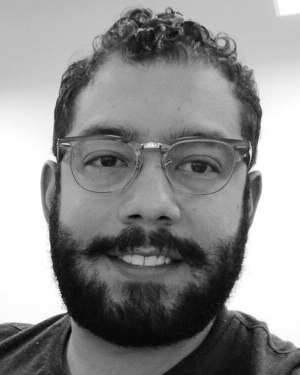
\includegraphics[width=1in,height=1.25in,clip,keepaspectratio]{../biography/yarib_300_375.jpg}}]{Yarib Nevarez} received the B.E. (Hons) degree in electronics from the Durango Institute of Technology, Durango, Mexico, in 2009, and the M.Sc. degree in Embedded Systems Design from the University of Applied Sciences Bremerhaven, Bremen, Germany, in 2017. He is currently pursuing a PhD degree with the Institute of Electrodynamics and Microelectronics, University of Bremen, Germany. His research interest is focused mainly on System-on-Chip architectures and hardware implementation for deep learning accelerators in Embedded Systems.
\\
During his professional experience, he served as a Senior Embedded Software Engineer at Texas Instruments, IBM, Continental Automotive, TOSHIBA, and Carbon Robotics. He has designed and developed software architectures for graphic calculators, automotive systems, robotic drivers, and more.
	
\end{IEEEbiography}

\begin{IEEEbiography}[{
\includegraphics[width=1in,height=1.25in,clip,keepaspectratio]{../biography/person.png}}]{ANDREAS BEERING}
\end{IEEEbiography}

\begin{IEEEbiography}[{
\includegraphics[width=1in,height=1.25in,clip,keepaspectratio]{../biography/person.png}}]{Amir Najafi}
\end{IEEEbiography}

\begin{IEEEbiography}[{
\includegraphics[width=1in,height=1.25in,clip,keepaspectratio]{../biography/person.png}}]{Ardalan Najafi}
\end{IEEEbiography}

\begin{IEEEbiography}[{
\includegraphics[width=1in,height=1.25in,clip,keepaspectratio]{../biography/person.png}}]{KARL-LUDWIG KRIEGER}
\end{IEEEbiography}

\begin{IEEEbiography}[{
\includegraphics[width=1in,height=1.25in,clip,keepaspectratio]{../biography/Alberto_Garcia-Ortiz.jpg}}]{Alberto Garcia-Ortiz}
    obtained the diploma degree in
    Telecommunication Systems from the Polytechnic University of
    Valencia (Spain) in 1998. After working for two years at Newlogic
    in Austria, he started the Ph.D. at the Institute of
    Microelectronic Systems, Darmstadt University of Technology,
    Germany. In 2003, he received from the Department of Electrical
    Engineering and Information Technology of the university the
    Ph.D. degree with "summa cum laude." From 2003 to 2005, he worked
    as a Senior Hardware Design Engineer at IBM Deutschland
    Development and Research in B{\"o}blingen.  After that he joined the
    start-up AnaFocus (Spain), where he was responsible for the design
    and integration of AnaFocus" next generation Vision
    Systems-on-Chip. He is currently full professor for the chair of
    integrated digital systems at the university of Bremen.
    Dr. Garcia-Ortiz received the "Outstanding dissertation award" in
    2004 from the European Design and Automation Association. In 2005,
    he received from IBM an innovation award for contributions to
    leakage estimation. Two patents are issued with that work. He
    serves as editor of JOLPE and is reviewer of several conferences,
    journals, and European projects. \\
    His interests include low-power
    design and estimation, communication- centric design, SoC
    integration, and variations-aware design. 
\end{IEEEbiography}
